\documentclass[conference]{IEEEtran}

\usepackage[utf8]{inputenc}
\usepackage[T1]{fontenc}
\usepackage[spanish,es-nodecimaldot]{babel}
\usepackage{amsmath}
\usepackage{booktabs}
\usepackage{graphicx}
\usepackage{hyperref}
\usepackage{microtype}
\usepackage{xcolor}
\usepackage{placeins}
\usepackage{tabularx}
\usepackage{balance}

\graphicspath{{figures/}}
\hypersetup{
    colorlinks=true,
    linkcolor=black,
    citecolor=black,
    urlcolor=blue
}

\title{¿Cómo se relaciona la ubicación geográfica de una vivienda en Medellín con su precio de venta?}

\author{
\IEEEauthorblockN{Kevin Arley Parra Henao}
\IEEEauthorblockA{
Universidad Nacional de Colombia, sede Medellín\\
Curso de Análisis Geoespacial
}
}

\begin{document}

\maketitle

\begin{abstract}
En este trabajo se analiza cómo se relaciona la ubicación geográfica de una vivienda en Medellín con su precio de venta. Se parte de un conjunto de datos de la plataforma Kaggle que contiene información sobre inmuebles en Colombia, como el número de habitaciones, dormitorios y baños, su ubicación y su precio de venta, entre otros datos. El precio está expresado en pesos colombianos. Para aplicar los modelos estudiados, se realizó la limpieza, el filtrado, el procesamiento y la normalización de los datos. Asimismo, se utilizó el logaritmo natural del precio para estabilizar los análisis. Los inmuebles se representaron como puntos marcados y se estudiaron mediante técnicas de análisis geoespacial. También se utilizaron métodos de aprendizaje automático, como Random Forest, para comparar sus resultados con los de los modelos espaciales. El precio logarítmico presentó dependencia espacial positiva y significativa ($I$ de Moran de 0.5898 con diez vecinos, $p=0.001$). El modelo SAR-Lag confirmó una relación positiva con los precios vecinos ($\rho=0.5496$), mientras que MGWR y el modelo jerárquico mostraron que el efecto de los atributos y el nivel base del precio cambian entre zonas y barrios. En la evaluación, Random Forest fue el modelo con mayor capacidad predictiva ($R^2=0.7756$ y RMSE de 0.3485 en escala logarítmica); entre los modelos espaciales interpretables, SAR-Lag fue el mejor ($R^2=0.5997$). Por tanto, la ubicación se relaciona con el precio mediante el contexto barrial, la semejanza entre viviendas cercanas y la variación territorial de las relaciones.
\end{abstract}


\section{Introducción}

El precio de una vivienda no depende únicamente de sus características como el número de habitaciones, la cantidad de dormitorios o el número de baños. Dos inmuebles similares pueden tener precios diferentes si se encuentran en barrios distintos. La accesibilidad, la seguridad, los servicios cercanos, la calidad del entorno y la valoración de cada sector ayudan a explicar esa diferencia. Además, las viviendas cercanas suelen compartir condiciones de mercado y, por esta razón, sus precios pueden parecerse.

Este comportamiento se estudia mediante dos conceptos. La \emph{dependencia espacial} aparece cuando el precio de una vivienda se relaciona con los precios de las viviendas cercanas. La \emph{heterogeneidad espacial} aparece cuando una característica no se relaciona de la misma manera con el precio en toda la ciudad. Por ejemplo, un baño adicional puede tener una relación más fuerte con el precio en una zona que en otra.

Este trabajo hace parte del proyecto realizado para la materia de análisis geoespacial, de la Universidad Nacional de Colombia. Los materiales del curso presentan métodos para estudiar estas dos dimensiones, desde patrones de puntos y autocorrelación hasta modelos locales, jerárquicos y procesos gaussianos \cite{materialcurso,librocurso}. Con base en estos métodos, el proyecto responde dos preguntas: ¿cómo se relaciona la ubicación geográfica de una vivienda en Medellín con su precio?, y ¿cómo la ubicación y la cercanía de inmuebles vecinos ayudan a explicar y predecir su precio de venta?

El objetivo consiste en describir el patrón territorial del precio, medir la dependencia espacial, evaluar si las relaciones cambian entre zonas y comparar métodos de predicción. El análisis no busca establecer relaciones causales. Los resultados muestran asociaciones espaciales y permiten establecer cuánto aporta cada método a la explicación o predicción del precio.

\section{Datos y metodología}

\subsection{Datos y representación espacial}

Los datos se descargaron directamente desde Kaggle a partir del conjunto \emph{Colombia Housing Properties Price} \cite{dataset}. Cada observación corresponde a un anuncio inmobiliario y la variable original \texttt{price} contiene el precio de venta anunciado en pesos colombianos. Para construir el conjunto de análisis, se seleccionaron las columnas útiles, se filtraron los anuncios correspondientes a la ciudad de Medellín y se conservaron únicamente las operaciones de venta. También se eliminaron las columnas constantes o sin información para la ciudad, como los niveles \texttt{l5} y \texttt{l6}, además del título del anuncio.

De los 119\,394 anuncios de venta identificados en Medellín, se eliminaron los registros sin coordenadas o sin precio. Para reducir el efecto de los valores extremos, se conservaron los precios entre los percentiles 1 y 99. El conjunto final contiene 35\,814 anuncios, con precios entre 82 y 4,200 millones de pesos y una mediana de 420 millones. Los datos se dividieron una sola vez en 25\,069 observaciones de entrenamiento (70\,\%) y 10\,745 de prueba (30\,\%), con semilla 42.

Los valores numéricos faltantes se imputaron con la mediana del conjunto de entrenamiento y después se estandarizaron con media cero y desviación estándar uno. Los valores categóricos faltantes se imputaron con la categoría más frecuente. El barrio y el tipo de propiedad se codificaron mediante variables indicadoras (One Hot Encoding). Todo el preprocesamiento se ajustó solo con los datos de entrenamiento y luego se aplicó a prueba para evitar fuga de información. Las variables de superficie tenían pocos datos disponibles; por esto, se usaron en los modelos generales de aprendizaje automático, pero no en los modelos espaciales explicativos.

Las variables empleadas incluyen precio, longitud, latitud, barrio, tipo de propiedad, habitaciones, dormitorios y baños. El precio original se conservó para describir resultados en pesos. Debido a su asimetría, para la etapa espacial se creó una variable adicional:
\begin{equation*}
    y_i=\log(\text{precio}_i).
\end{equation*}
El logaritmo reduce la influencia de las viviendas muy costosas y facilita la comparación de cambios relativos. Esta transformación no reemplaza ni modifica el precio original y sigue el tratamiento presentado en el material del curso \cite{materialcurso}.

Los anuncios se representaron como puntos y se proyectaron en MAGNA-SIRGAS / Origen-Nacional (EPSG:9377), un sistema cuyas unidades están en metros. Como algunos registros etiquetados como Medellín se encontraban fuera del municipio, el análisis espacial conservó únicamente los puntos dentro de sus límites. La unión espacial con 252 polígonos del material del curso asignó 22\,857 puntos de entrenamiento a 226 barrios con al menos un anuncio. GWR, MGWR y los modelos continuos utilizaron muestras de estas geometrías para controlar el costo computacional.

El código utilizado para el procesamiento, los modelos y la generación de las figuras está disponible en el repositorio del proyecto en la plataforma GitHub \cite{repositorio}.

\subsection{Patrón de puntos y agrupamiento}

Cada anuncio se trató como un punto marcado por su precio. Se calcularon el centro medio, el centro ponderado por \texttt{log\_price}, la elipse de desviación estándar y la envolvente convexa. La superficie kernel normalizada se definió como:
\begin{equation*}
    \widehat{m}(s)=
    \frac{\sum_i K_h(s-s_i)y_i}
         {\sum_i K_h(s-s_i)},
\end{equation*}
con un ancho de banda de 1 km. La normalización permite separar la cantidad de anuncios del nivel local del precio. La formulación se basa en el capítulo de patrones de puntos del libro del curso \cite{librocurso}.

K-means se ajustó únicamente con las coordenadas proyectadas y estandarizadas. Se probaron entre dos y seis grupos. Silhouette mide qué tan compactos y separados están los grupos. El método del codo muestra cuándo agregar más clusters deja de reducir de forma importante la inercia.

\subsection{Dependencia espacial}

Para los puntos se construyeron matrices de vecinos más cercanos (KNN) con 5, 10 y 20 vecinos. En este análisis, $k$ indica cuántos vecinos se consideran alrededor de cada vivienda y no el número de grupos de K-means. Moran global mide si los valores cercanos tienden a parecerse. Un resultado positivo y significativo indica agrupación de valores similares. Moran local o LISA muestra dónde se encuentra ese patrón:
\begin{itemize}
    \item Alto--Alto: precio alto rodeado por precios altos.
    \item Bajo--Bajo: precio bajo rodeado por precios bajos.
    \item Alto--Bajo y Bajo--Alto: observaciones que contrastan con su entorno.
\end{itemize}

Para los barrios se utilizó una matriz Queen, en la que dos barrios son vecinos si comparten un borde o un vértice. Moran y LISA se calcularon sobre la mediana barrial de \texttt{log\_price}, con 999 permutaciones.

OLS se empleó como modelo global de referencia:
\begin{equation*}
    \mathbf{y}=\mathbf{X}\boldsymbol{\beta}+\boldsymbol{\varepsilon}.
\end{equation*}
La notación de OLS y de los modelos espaciales se basa en los contenidos de correlación y regresión espacial del libro y del material del curso \cite{librocurso,materialcurso}. Después se ajustaron SEM y SAR. SEM representa la dependencia asociada con factores espaciales no incluidos:
\begin{equation*}
    \mathbf{u}=\lambda\mathbf{W}\mathbf{u}+\boldsymbol{\varepsilon}.
\end{equation*}
SAR incorpora el precio de las viviendas vecinas:
\begin{equation*}
    \mathbf{y}=\rho\mathbf{W}\mathbf{y}
    +\mathbf{X}\boldsymbol{\beta}+\boldsymbol{\varepsilon}.
\end{equation*}

Como referencia predictiva se ajustaron Random Forest y XGBoost con las variables procesadas. Estos métodos se usaron como contraste no espacial para comparar los modelos espaciales con algoritmos de otra familia. Sus hiperparámetros se eligieron mediante validación cruzada dentro del entrenamiento y la evaluación final se realizó sobre las mismas 10\,745 observaciones de prueba. Estos modelos miden cuánto puede predecirse, pero no describen directamente la dependencia o la heterogeneidad espacial ni producen un parámetro como $\rho$ en SAR-Lag.

\subsection{Heterogeneidad y regímenes espaciales}

GWR (\emph{Geographically Weighted Regression}) estima coeficientes alrededor de cada punto con un ancho de banda común. MGWR (\emph{Multiscale Geographically Weighted Regression}) permite un ancho diferente para cada variable:
\begin{equation*}
    y_i=\beta_0(s_i)+\sum_{k=1}^{p}\beta_k(s_i)x_{ik}+\varepsilon_i.
\end{equation*}
Esta formulación corresponde al desarrollo de GWR y MGWR presentado en el libro del curso \cite{librocurso}.

Se seleccionaron 1\,890 puntos distribuidos dentro de Medellín. Los predictores fueron número de habitaciones, número de dormitorios y número de baños estandarizados. El ancho de banda se seleccionó mediante AICc, un criterio que compara el ajuste y la complejidad y penaliza los parámetros innecesarios. También se evaluaron la significancia local, el número de condición y Moran residual.

Para representar los barrios como regímenes se compararon OLS, un modelo de intercepto aleatorio y un modelo con intercepto y pendiente aleatorios de baños. El ICC se calculó como:
\begin{equation*}
    \mathrm{ICC}=
    \frac{\sigma^2_{\text{barrio}}}
    {\sigma^2_{\text{barrio}}+\sigma^2_{\text{residual}}}.
\end{equation*}
Este valor indica qué proporción de la variación restante corresponde a diferencias entre barrios. La definición del ICC y la estructura jerárquica siguen el capítulo de modelos jerárquicos del libro \cite{librocurso}.

\subsection{Interpolación y validación espacial}

Se construyeron 38 bloques espaciales de aproximadamente 2 km. De los puntos usados, 1\,646 quedaron para entrenamiento y 244 para prueba. Ningún bloque de prueba apareció en entrenamiento, por lo que la evaluación representa la predicción en zonas completas no observadas.

Kriging ordinario predice a partir de los valores cercanos y de un variograma. Se compararon los modelos esférico, exponencial y gaussiano, con un máximo de 80 vecinos. Regresión-Kriging primero estimó la tendencia con habitaciones, dormitorios y baños mediante Ridge y después interpoló los residuos.

El proceso gaussiano utilizó un kernel Matérn con ruido blanco:
\begin{equation*}
    k(s_i,s_j)=\sigma_f^2
    k_{\mathrm{Mat\acute ern}\,3/2}(s_i,s_j)
    +\sigma_n^2\delta_{ij}.
\end{equation*}
La representación mediante funciones de covarianza y ruido se basa en los capítulos de Kriging y procesos gaussianos del libro y en el material del curso \cite{librocurso,materialcurso}. La media posterior corresponde a la predicción y la desviación estándar posterior mide su incertidumbre. Los métodos se compararon con $R^2$, MAE, RMSE y Moran residual.

\section{Resultados}

\subsection{Patrón espacial y barrios}

La Fig.~\ref{fig:marked-points} presenta cada vivienda como un punto marcado usando el precio logarítmico como marca. Los anuncios se concentran principalmente en la zona central, el occidente y el sur de Medellín. Los valores altos aparecen con mayor frecuencia en el suroriente, especialmente en El Poblado. El logaritmo permite observar este patrón sin que unos pocos precios extremos controlen la escala de color. Las zonas con pocos puntos tienen menor cobertura de anuncios y no necesariamente menos viviendas.

\begin{figure}[!t]
    \centering
    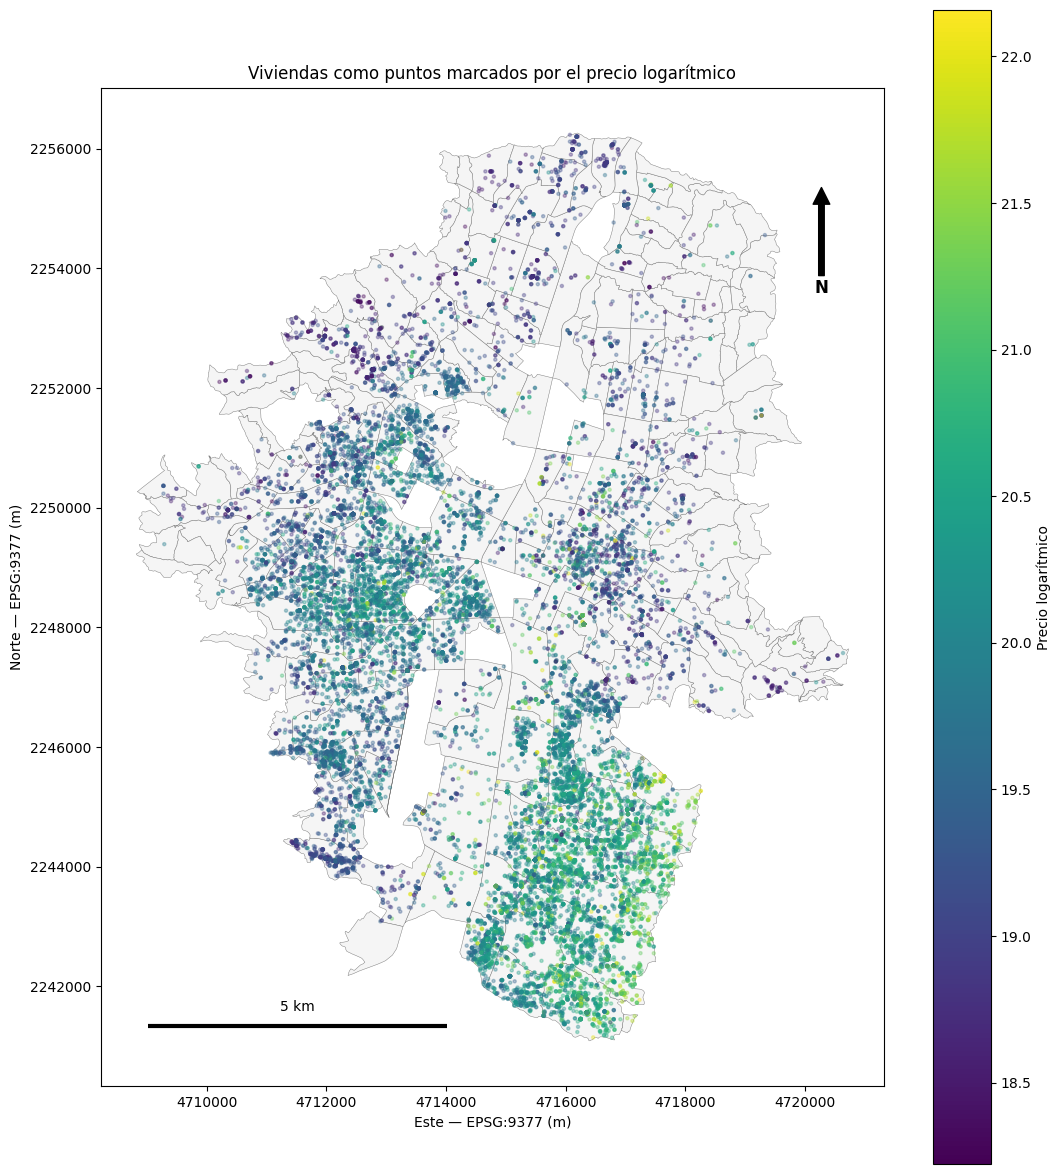
\includegraphics[width=\columnwidth]{marked_points.png}
    \caption{Viviendas como puntos marcados por el precio logarítmico. El mapa conserva las coordenadas EPSG:9377, la escala gráfica, el norte y los límites barriales.}
    \label{fig:marked-points}
\end{figure}

El centro medio se ubicó en Tenche y el centro ponderado por precio en Trinidad. La distancia entre ambos fue de 65.02 m. Este desplazamiento pequeño indica que los anuncios costosos del suroriente no cambian de forma importante el centro general, porque la oferta también se distribuye por el centro, el occidente y el norte. La elipse presentó semiejes de 3.38 km y 1.81 km, con una orientación de 105.33 grados, consistente con la forma alargada del valle.

\begin{figure}[!t]
    \centering
    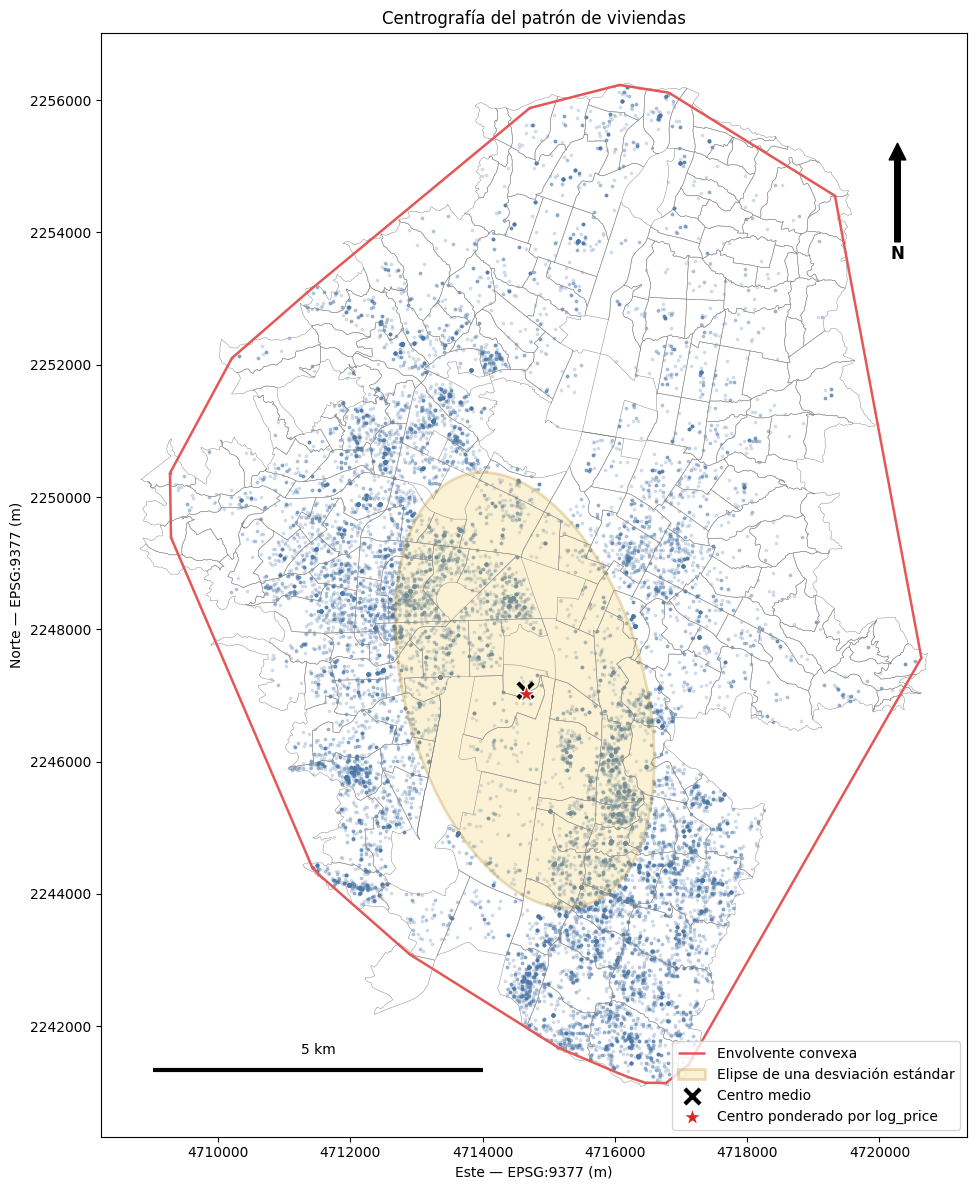
\includegraphics[width=\columnwidth]{centrography.png}
    \caption{Centrografía del patrón de anuncios. La cruz es el centro medio, la estrella es el centro ponderado por precio, la elipse resume dispersión y la línea roja muestra la envolvente convexa.}
    \label{fig:centrography}
\end{figure}

La superficie kernel varió aproximadamente entre 19.00 y 20.64 en escala logarítmica, equivalentes a valores cercanos a 178 y 922 millones de pesos. Los máximos se concentraron hacia El Poblado y representan precios locales promedio más altos, no una mayor cantidad de anuncios.

Una zona con muchos puntos no necesariamente presenta el mayor precio local, porque la superficie divide la suma ponderada del precio por la densidad de anuncios. Las zonas sin soporte suficiente no se estiman y, por tanto, no representan precios bajos.

K-means seleccionó tres clusters con un Silhouette de 0.520. El cluster 0 agrupó viviendas del centro y del norte, como La Candelaria y Boston, con una mediana en el precio de 250 millones. El cluster 1 cubrió gran parte del occidente, incluidos Laureles, Los Conquistadores y Belén, con mediana 340 millones. El cluster 2 reunió principalmente sectores de El Poblado, como El Tesoro, San Lucas, Los Balsos y Castropol, y alcanzó 690 millones. El precio no se utilizó para crear los grupos; las diferencias se calcularon después de agrupar los puntos por su ubicación.

\begin{figure*}[!t]
    \centering
    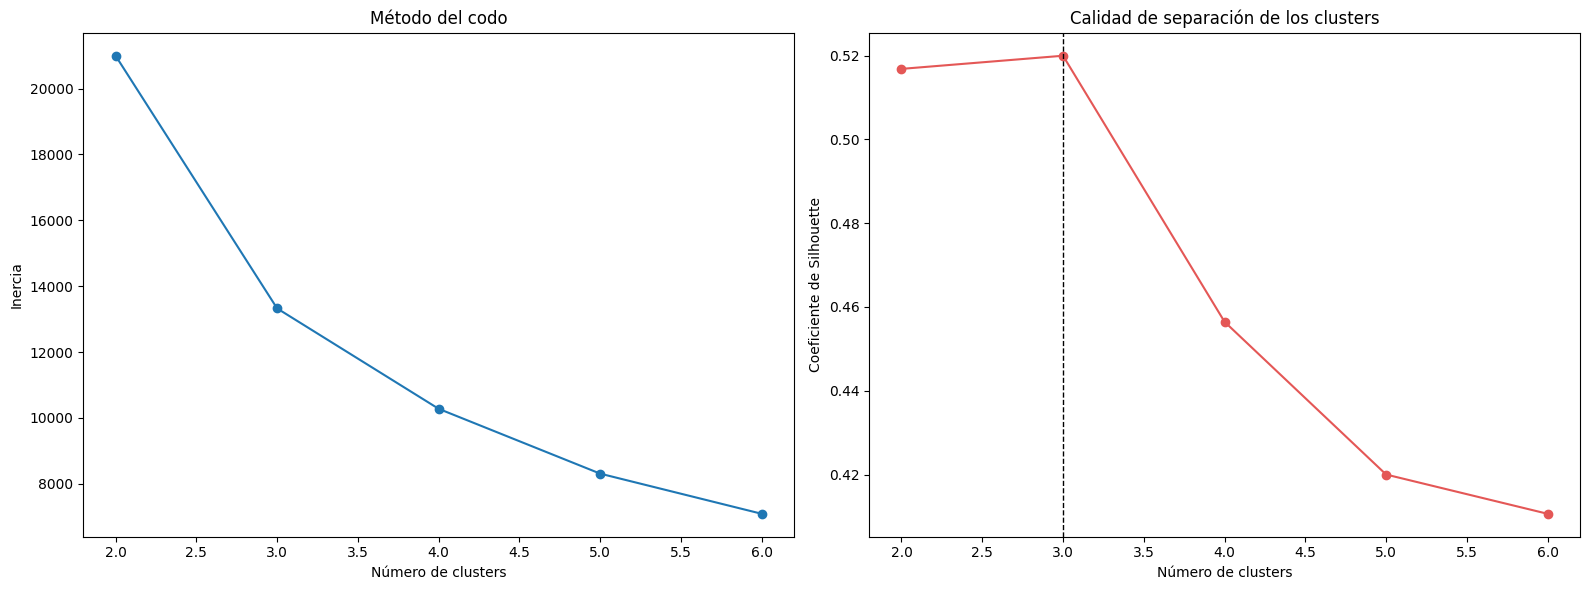
\includegraphics[width=0.94\textwidth]{kmeans_selection.png}
    \caption{Selección del número de clusters. El panel izquierdo muestra el método del codo y el derecho el coeficiente Silhouette para valores de $k$ entre 2 y 6.}
    \label{fig:kmeans-selection}
\end{figure*}

\begin{figure}[!t]
    \centering
    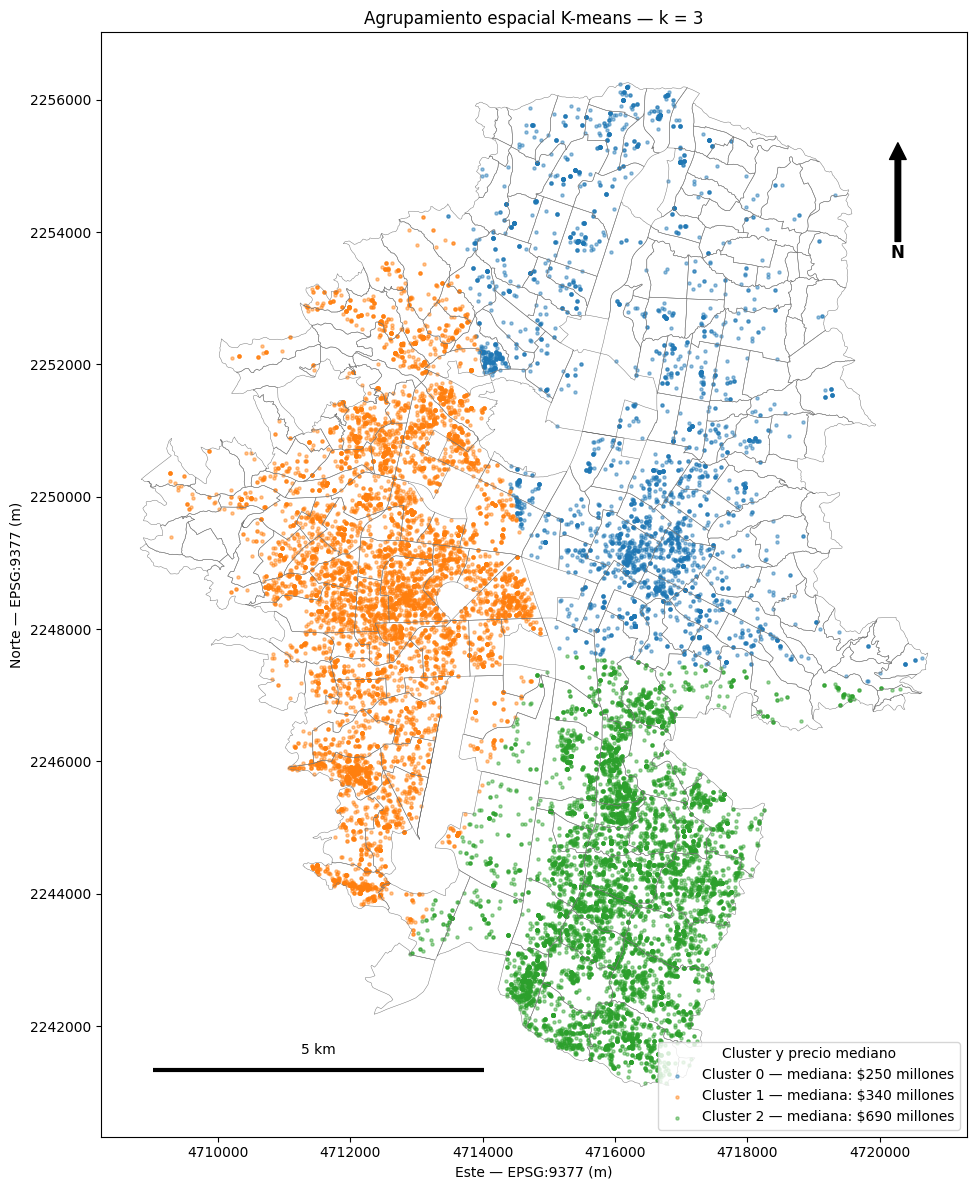
\includegraphics[width=\columnwidth]{spatial_kmeans.png}
    \caption{Agrupamiento espacial K-means con $k=3$. Los grupos se construyen únicamente con las coordenadas; la leyenda presenta el precio mediano calculado después del agrupamiento.}
    \label{fig:kmeans}
\end{figure}

La Fig.~\ref{fig:kmeans-selection} explica la selección del valor de tres para los grupos k-means: en este punto aparece el mayor Silhouette y la reducción de la inercia empieza a ser menor. La Fig.~\ref{fig:kmeans} muestra su distribución en Medellín. Las diferencias entre medianas indican que la ubicación permite identificar zonas con mercados distintos. Sin embargo, los clusters son regiones estadísticas definidas por cercanía a centroides; no reemplazan los barrios ni demuestran que la ubicación cause el precio.

Las coropletas de la Fig.~\ref{fig:choropleths} muestran el precio y la cantidad de anuncios por barrio. El mapa izquierdo muestra medianas mayores en el sur y el suroriente, mientras gran parte del norte presenta valores menores. El mapa derecho muestra una densidad desigual, concentrada en algunos barrios del centro, el occidente y el sur. Un barrio oscuro en el mapa de densidad no es necesariamente más costoso; solo tiene más anuncios por unidad de área. Las áreas blancas no cuentan con información suficiente en la muestra.

\begin{figure*}[!t]
    \centering
    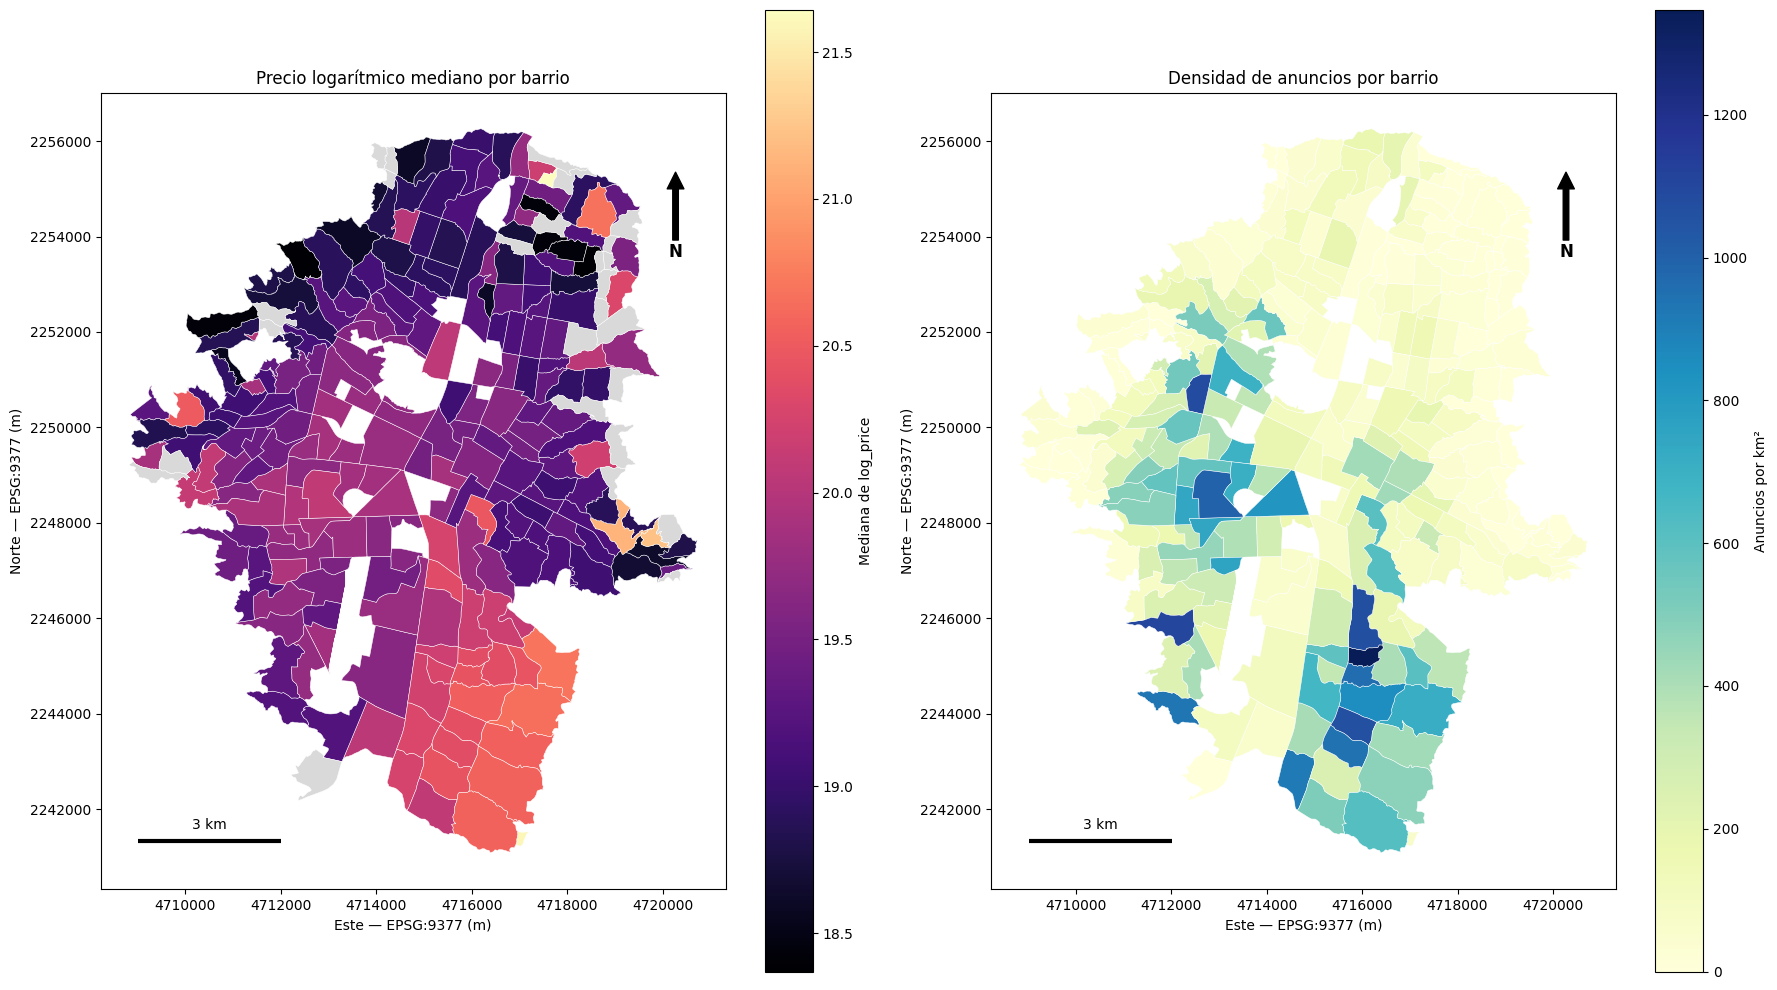
\includegraphics[width=0.96\textwidth]{neighborhood_choropleths.png}
    \caption{Resultados por barrio. Izquierda: precio logarítmico mediano. Derecha: densidad de anuncios por kilómetro cuadrado.}
    \label{fig:choropleths}
\end{figure*}

\subsection{Dependencia espacial global y local}

Los resultados confirman dependencia espacial. Moran fue 0.6254 para $k=5$, 0.5898 para $k=10$ y 0.5553 para $k=20$; en los tres casos, $p=0.001$. Los valores positivos y significativos indican que las viviendas cercanas tienden a presentar precios similares. Moran disminuye al incluir más vecinos porque la relación es más fuerte en el entorno inmediato y se suaviza al ampliar el vecindario. Aun así, la dependencia permanece con veinte vecinos. En este análisis, $k$ corresponde a KNN y no a los tres clusters de K-means.

LISA puntual clasificó 23.81\,\% de las viviendas como Alto--Alto y 24.44\,\% como Bajo--Bajo. Los casos Bajo--Alto representaron 3.23\,\% y los Alto--Bajo 2.09\,\%. A escala barrial, Moran fue 0.4752 ($p=0.001$). Se encontraron 29 barrios Alto--Alto, con una mediana conjunta de 690 millones, y 37 Bajo--Bajo, con 165 millones. El 46.4 \% no presenta asociación local significativa.

\begin{figure}[!t]
    \centering
    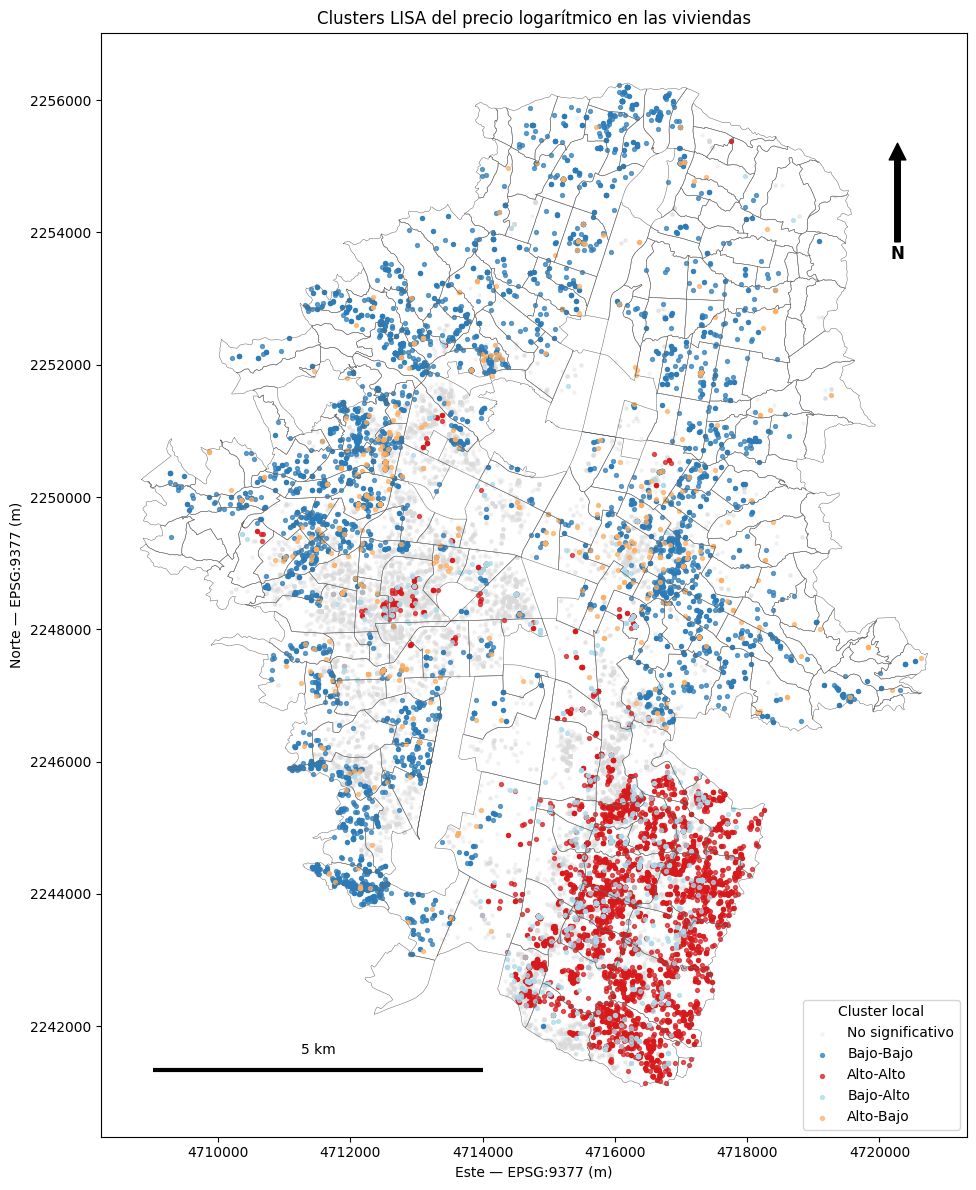
\includegraphics[width=\columnwidth]{point_lisa.png}
    \caption{Clusters LISA del precio logarítmico en las viviendas. Solo se clasifican asociaciones locales con $p<0.05$.}
    \label{fig:point-lisa}
\end{figure}

En la Fig.~\ref{fig:point-lisa}, Alto--Alto representa viviendas costosas rodeadas por otras costosas, mientras Bajo--Bajo representa viviendas de menor precio rodeadas por precios similares. Estos grupos muestran continuidad local del mercado. Alto--Bajo y Bajo--Alto son viviendas que contrastan con sus vecinos y aparecen con menor frecuencia. Los puntos no significativos no tienen evidencia suficiente para asignarles un patrón local.

\begin{figure}[!t]
    \centering
    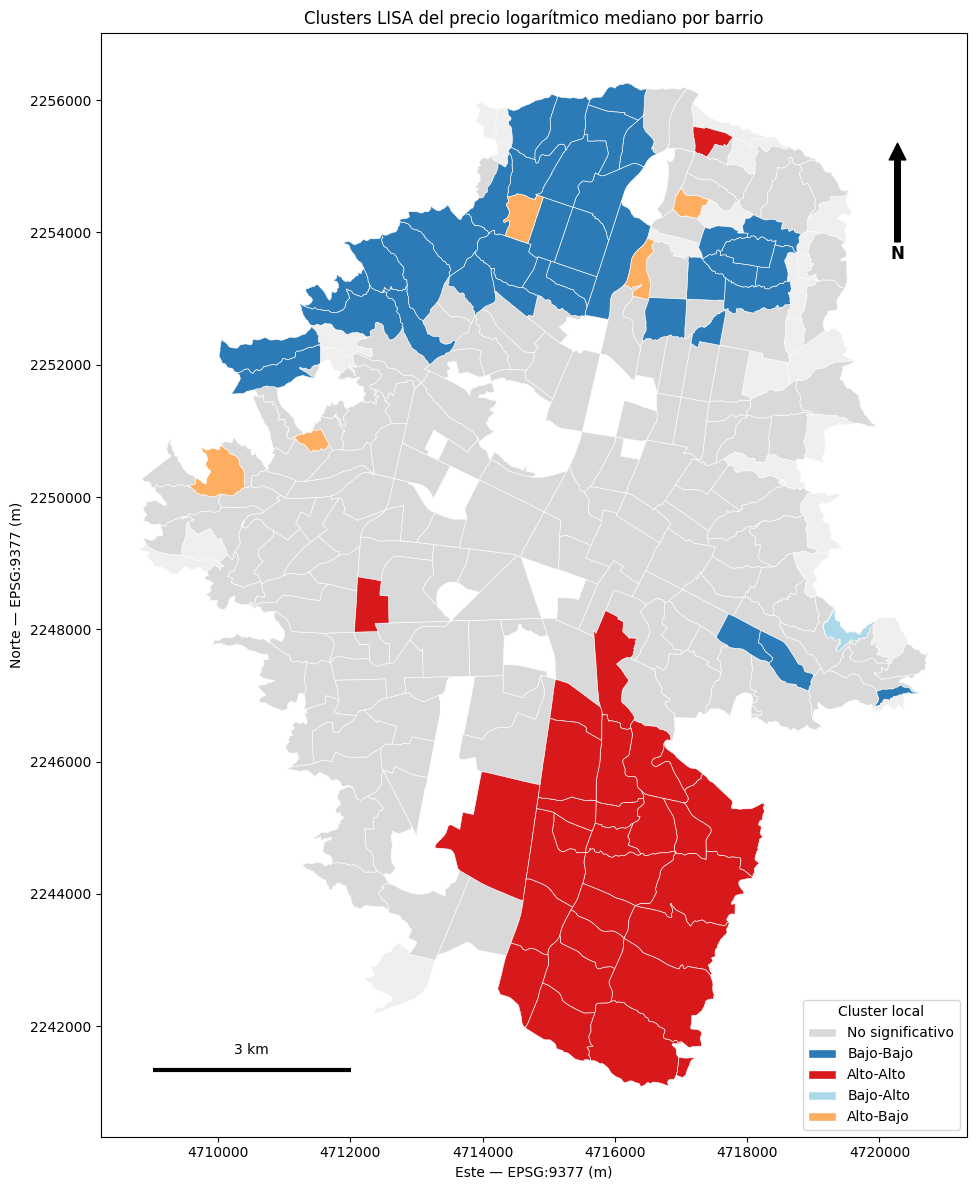
\includegraphics[width=\columnwidth]{neighborhood_lisa.png}
    \caption{Clusters LISA del precio logarítmico mediano por barrio. Rojo representa Alto--Alto y azul Bajo--Bajo.}
    \label{fig:lisa}
\end{figure}

La matriz Queen tuvo 4.86 vecinos por barrio, dos componentes conectados y ninguna isla. El componente principal incluyó 224 barrios. El segundo estuvo formado por María Cano--Carambolas y Carpinelo, que están conectados entre sí, pero no con los barrios observados del componente principal.

\subsection{Modelos globales y comparación predictiva}

OLS obtuvo $R^2=0.5870$ y RMSE de 0.4745 en entrenamiento. Sus residuos conservaron un Moran de 0.2461 ($p=0.001$), por lo que los atributos incluidos no explicaron toda la estructura territorial.

SEM estimó $\lambda=0.7351$ ($p<0.001$). Este valor indica que factores territoriales no incluidos presentan un patrón entre viviendas vecinas. Después de filtrar esta estructura, el error tuvo un Moran de $-0.0013$ y $p=0.243$, sin evidencia de dependencia restante.

SAR-Lag estimó $\rho=0.5496$ ($p<0.001$). El resultado indica una relación positiva entre el precio de una vivienda y los precios de sus vecinas. En prueba, fue el mejor modelo espacial global, con $R^2=0.5997$ y RMSE de 0.4655. Sin embargo, su Moran residual de 0.1753 muestra que todavía quedó estructura espacial sin explicar.

\begin{table}[!t]
\caption{Comparación común sobre precio logarítmico en prueba}
\label{tab:global}
\centering
\begin{tabular}{lccc}
\toprule
Modelo & $R^2$ & RMSE & Moran residual\\
\midrule
OLS & 0.5828 & 0.4752 & 0.1926\\
SEM & 0.5649 & 0.4853 & 0.2437\\
SAR-Lag & 0.5997 & 0.4655 & 0.1753\\
Random Forest & \textbf{0.7756} & \textbf{0.3485} & \textbf{0.0293}\\
XGBoost & 0.5944 & 0.4686 & 0.0790\\
\bottomrule
\end{tabular}
\end{table}

Random Forest obtuvo el mejor desempeño general y la menor autocorrelación residual. Por esto, fue el mejor predictor entre los modelos evaluados. SAR-Lag tuvo menor precisión, pero respondió de forma más directa a la pregunta espacial, porque $\rho$ cuantifica la relación entre el precio de una vivienda y los precios de sus vecinas. Los dos resultados muestran que precisión e interpretación son objetivos diferentes.

\subsection{Heterogeneidad espacial}

\begin{table}[!t]
\caption{Comparación de heterogeneidad sobre 1\,890 puntos}
\label{tab:heterogeneity}
\centering
\begin{tabular}{lcccc}
\toprule
Modelo & $R^2$ aj. & AICc & RMSE & Moran\\
\midrule
OLS & 0.3758 & --- & 0.6129 & 0.2722\\
GWR & 0.5985 & 2837.88 & 0.4738 & 0.0132\\
MGWR & \textbf{0.6102} & \textbf{2773.17} & \textbf{0.4678} & -0.0347\\
\bottomrule
\end{tabular}
\end{table}

MGWR obtuvo el mejor equilibrio entre ajuste y complejidad. Los anchos de banda fueron 64 vecinos para el intercepto, 1\,015 para habitaciones, 364 para dormitorios y 149 para baños. El ancho de habitaciones indica una relación amplia y estable. Los anchos menores del intercepto y de baños permiten cambios más locales.

Baños presentó un efecto positivo y significativo en 83.54\,\% de los puntos, habitaciones en 54.07\,\% y dormitorios en 5.03\,\%. El coeficiente local de baños varió entre 0.154 y 0.747. Por tanto, existe heterogeneidad: la relación es positiva, pero su intensidad cambia entre zonas. El número de condición estuvo entre 1.5 y 3.2 y ningún punto superó 30, por lo que no se encontró multicolinealidad local fuerte.

\begin{figure*}[!t]
    \centering
    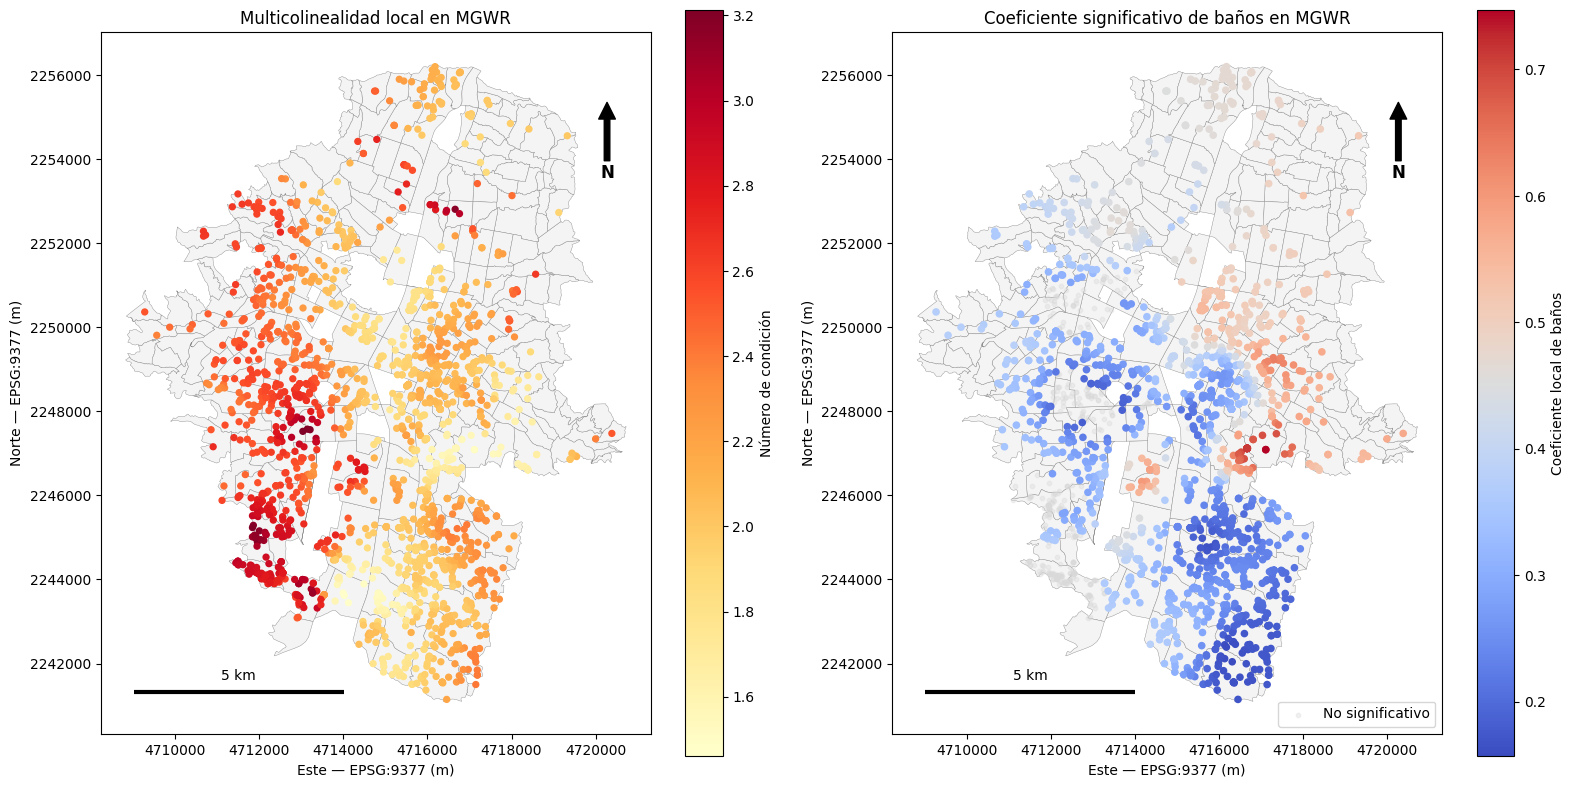
\includegraphics[width=0.94\textwidth]{mgwr_diagnostics.png}
    \caption{Diagnósticos MGWR. Izquierda: número de condición local. Derecha: coeficientes significativos de baños; los puntos grises no fueron significativos.}
    \label{fig:mgwr}
\end{figure*}

GWR redujo Moran residual a 0.0132 con $p=0.084$, sin evidencia de dependencia al nivel de 5\,\%. MGWR produjo un valor pequeño y negativo de $-0.0347$ ($p=0.001$). Ambos modelos captaron casi toda la agrupación positiva inicial, aunque MGWR dejó una alternancia local leve.

\begin{figure}[!htbp]
    \centering
    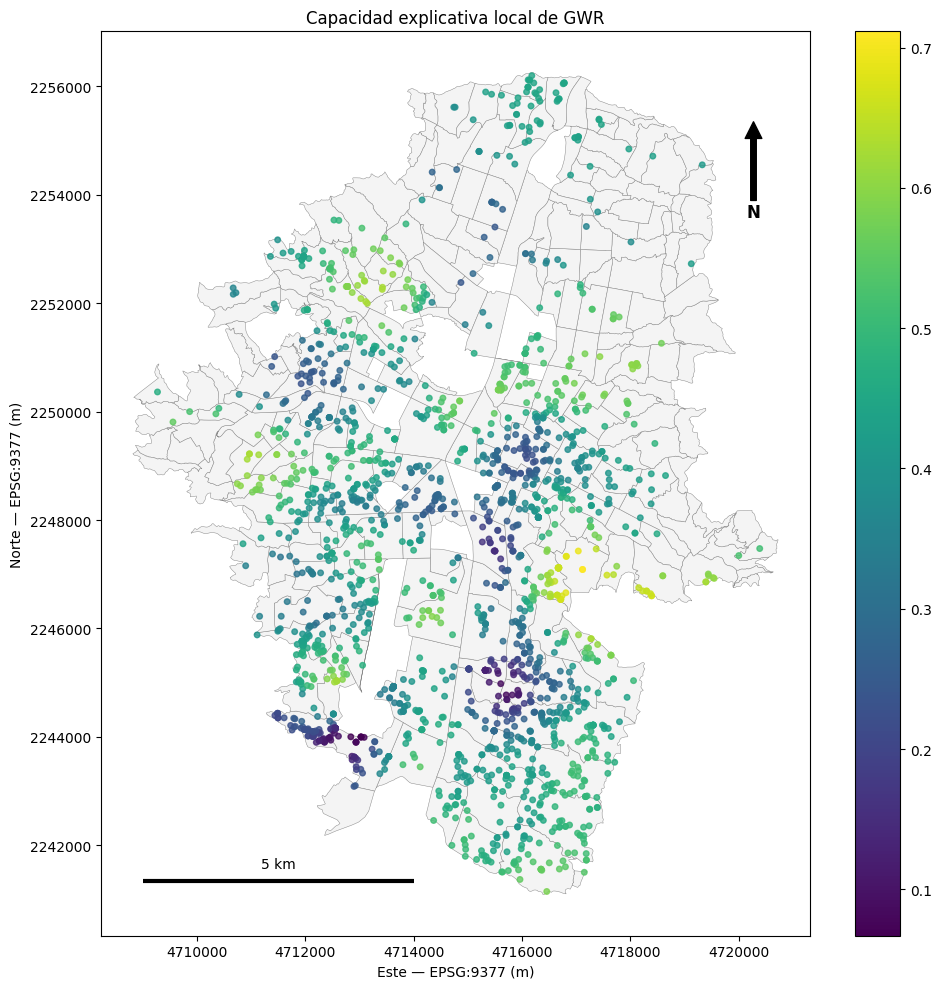
\includegraphics[width=\columnwidth]{gwr_local_r2.png}
    \caption{Capacidad explicativa local de GWR. El color representa el $R^2$ calculado alrededor de cada punto.}
    \label{fig:gwr-r2}
\end{figure}

El $R^2$ local de la Fig.~\ref{fig:gwr-r2} varía entre 0.07 y 0.71. Los valores altos indican que habitaciones, dormitorios y baños explican una mayor proporción de la variación del precio en ese entorno. Los valores bajos no representan precios bajos, sino zonas donde el modelo explica menos y probablemente faltan variables territoriales o estructurales. El ajuste fue mayor en sectores del centro-occidente, centro-oriente y suroriente, y menor en partes de Guayabal y del suroccidente.

\subsection{Regímenes por barrio}

El modelo de intercepto aleatorio estimó varianza entre barrios de 0.182 y varianza residual de 0.1963. De estas cifras se obtuvo un ICC de 0.4809:
\begin{equation*}
    \mathrm{ICC}=\frac{0.182}{0.182+0.1963}=0.4809.
\end{equation*}
El resultado indica que 48.1\,\% de la variación restante se encuentra entre barrios y 51.9\,\% entre viviendas del mismo barrio.

El modelo con intercepto y pendiente aleatoria de baños obtuvo el menor AIC (27\,755.80) y RMSE en muestra (0.4303). Mejoró al modelo de solo intercepto, con AIC de 28\,472.25 y RMSE de 0.4410, y al OLS comparable, con RMSE de 0.5773. Por tanto, los barrios difieren tanto en su nivel base de precio como en la relación entre baños y precio.

\begin{figure}[!htbp]
    \centering
    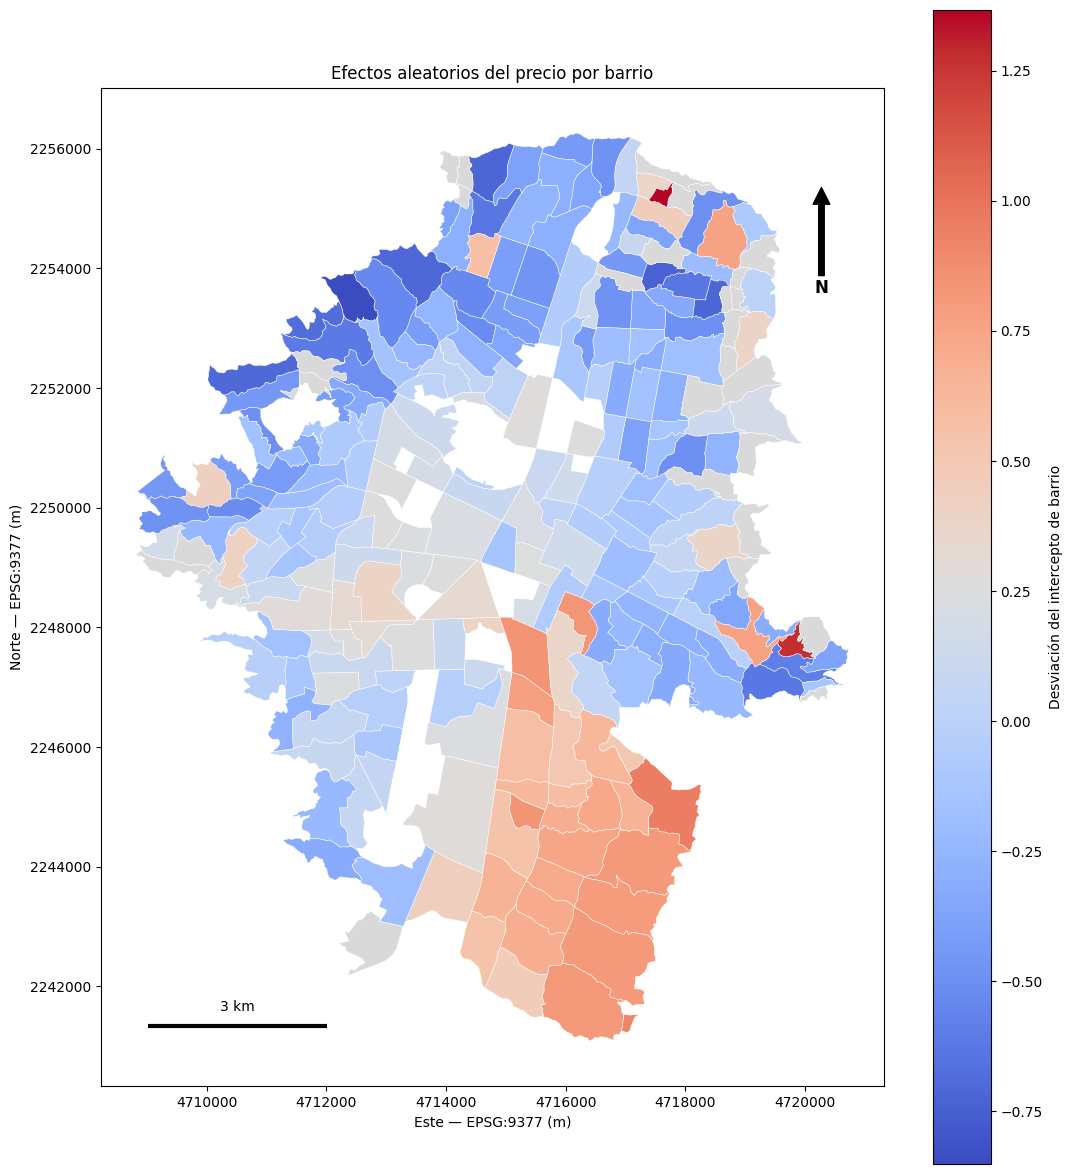
\includegraphics[width=\columnwidth]{hierarchical_effects.png}
    \caption{Efectos aleatorios del intercepto por barrio. Los tonos rojos indican un nivel base superior al promedio y los azules uno inferior, después de controlar los atributos incluidos.}
    \label{fig:hierarchical}
\end{figure}

\subsection{Kriging y procesos gaussianos}

El variograma esférico se seleccionó porque produjo el menor RMSE (0.5094), aunque las diferencias frente al exponencial (0.5128) y al gaussiano (0.5153) fueron pequeñas. El modelo estimó un nugget de 0.2742, un sill total de 1.0484 y un range de 12.75 km. El range indica hasta qué distancia se mantiene la relación espacial y el nugget representa diferencias muy locales o ruido.

\begin{figure}[!htbp]
    \centering
    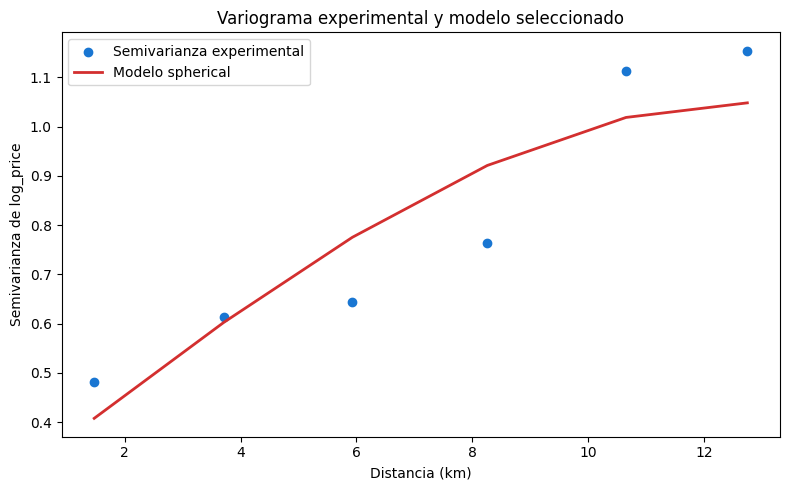
\includegraphics[width=0.88\columnwidth]{selected_variogram.png}
    \caption{Semivarianza experimental y variograma esférico seleccionado.}
    \label{fig:variogram}
\end{figure}

La semivarianza de la Fig.~\ref{fig:variogram} aumenta con la distancia. Esto indica que las viviendas más separadas tienden a diferir más en precio. La estabilización alrededor del sill muestra el punto en el que una mayor distancia aporta poca información. El nugget distinto de cero indica que incluso viviendas muy cercanas pueden presentar diferencias por atributos no observados o por ruido del anuncio.

El proceso gaussiano optimizó el kernel
\begin{multline*}
0.746^2 \times \mathrm{Mat\acute ern}
(\ell=[1.05,0.603],\\
\nu=1.5)+\mathrm{WhiteKernel}(0.595).
\end{multline*}
La varianza espacial fue 0.557 y el ruido 0.595. El ruido ligeramente mayor indica que una parte importante de la diferencia entre precios no se explica únicamente mediante una superficie espacial suave.

\begin{table}[!t]
\caption{Validación por bloques de modelos continuos}
\label{tab:continuous}
\centering
\begin{tabular}{lcccc}
\toprule
Modelo & $R^2$ & MAE & RMSE & Moran\\
\midrule
Kriging & 0.2256 & 0.3801 & 0.5094 & 0.1878\\
Reg.-Kriging & \textbf{0.4373} & \textbf{0.3116} & \textbf{0.4343} & 0.0657\\
Proceso gaussiano & 0.1610 & 0.3951 & 0.5302 & 0.2481\\
\bottomrule
\end{tabular}
\end{table}

Regresión-Kriging fue el mejor método continuo. Primero explicó parte del precio mediante los atributos de la vivienda y después utilizó la cercanía para interpolar los residuos. Su Moran residual de 0.0657 ($p=0.017$) fue menor que el de Kriging ordinario y el proceso gaussiano, aunque todavía fue significativo.

\begin{figure}[!htbp]
    \centering
    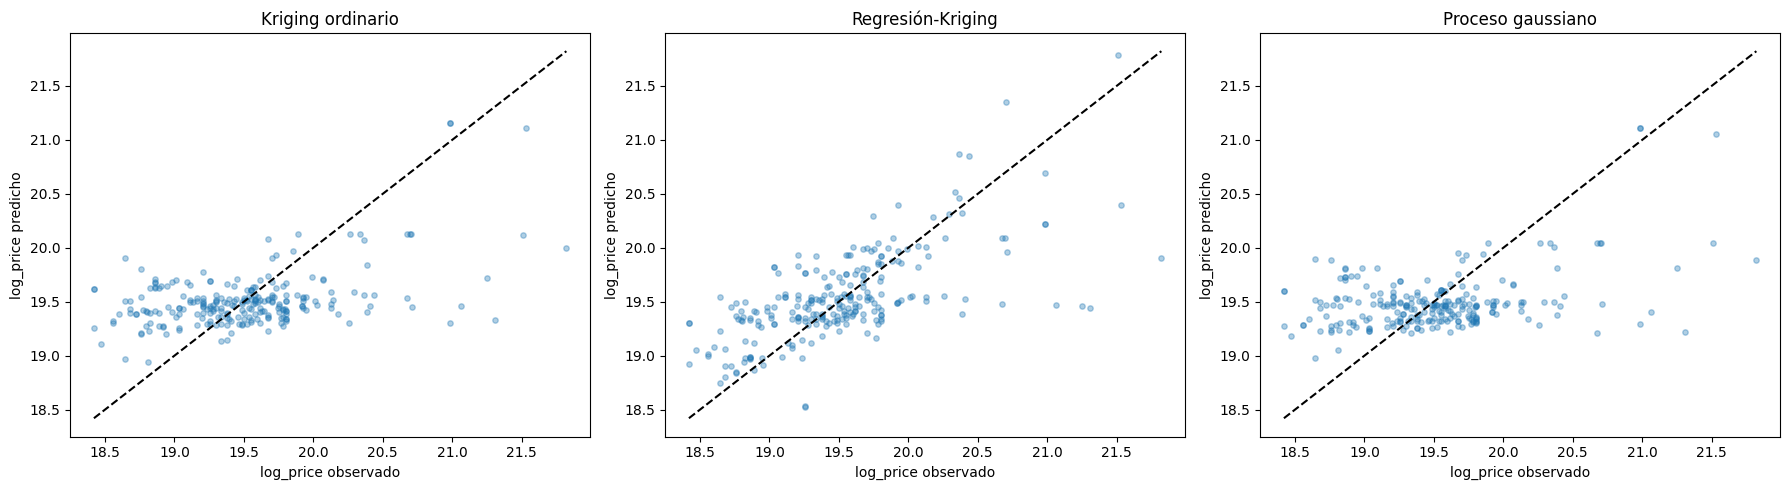
\includegraphics[width=\columnwidth]{continuous_validation.png}
    \caption{Predicción frente al valor observado bajo validación por bloques. Una mayor cercanía a la diagonal representa mejor correspondencia entre predicción y observación.}
    \label{fig:continuous-validation}
\end{figure}

La Fig.~\ref{fig:continuous-validation} muestra que Regresión-Kriging sigue mejor la diagonal y presenta menor dispersión. Kriging ordinario y el proceso gaussiano suavizan los extremos: sobreestiman algunos precios bajos y subestiman varios precios altos. Este comportamiento aparece cuando la predicción depende principalmente de una superficie espacial suave.

\begin{figure}[!htbp]
    \centering
    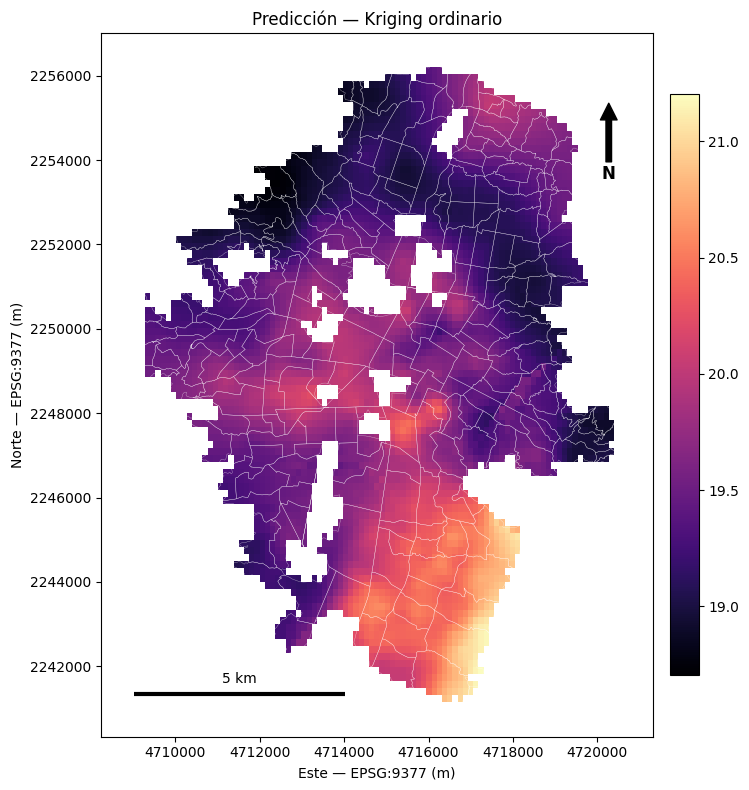
\includegraphics[width=0.78\columnwidth]{kriging_surface.png}
    \caption{Predicción de Kriging ordinario. Los precios esperados son mayores hacia El Poblado y el suroriente y menores hacia el norte.}
    \label{fig:surfaces}
\end{figure}

\begin{figure}[!htbp]
    \centering
    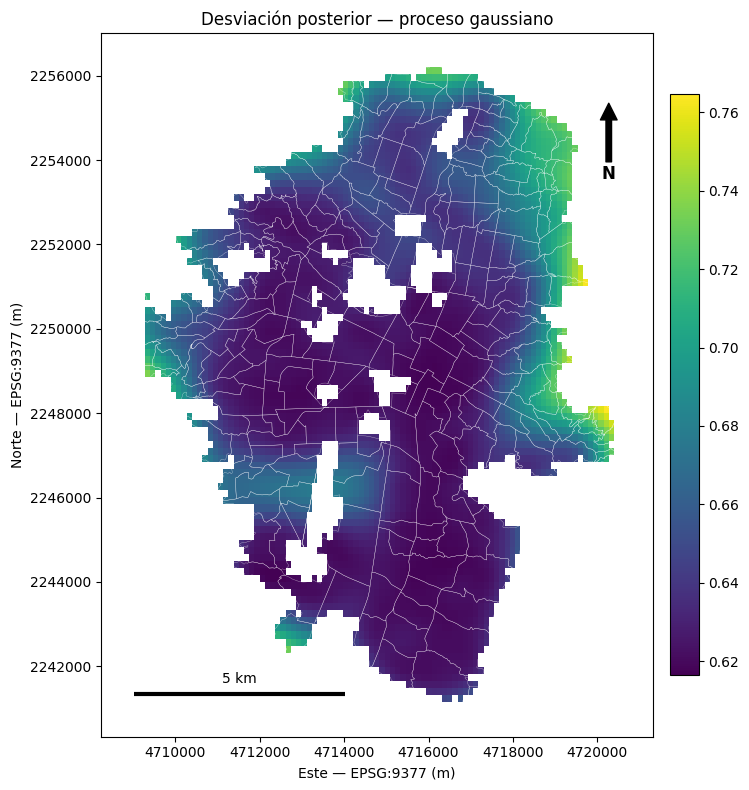
\includegraphics[width=0.78\columnwidth]{gaussian_uncertainty.png}
    \caption{Desviación estándar posterior del proceso gaussiano. Los valores altos representan mayor incertidumbre, no precios más altos.}
    \label{fig:gp-uncertainty}
\end{figure}

Kriging estimó precios más altos hacia El Poblado y el suroriente y valores menores hacia el norte. La incertidumbre media fue 0.5989 para Kriging, 0.5628 para Regresión-Kriging y 0.6624 para el proceso gaussiano. Una incertidumbre alta no representa un precio alto, sino menor evidencia para establecer la predicción, especialmente en las zonas periféricas.

La Fig.~\ref{fig:gp-uncertainty} muestra menor incertidumbre en las zonas centrales, donde existe mayor soporte de puntos. La incertidumbre aumenta hacia los bordes oriental y nororiental, porque el modelo debe extender el patrón aprendido desde observaciones más lejanas. En estas zonas, las predicciones deben interpretarse con mayor cautela.

\subsection{Comparación final de métodos}

La Tabla~\ref{tab:final-comparison} reúne los resultados obtenidos al ejecutar los modelos. Un $R^2$ mayor representa una mayor proporción explicada, un RMSE menor representa errores más pequeños y un $I$ de Moran residual cercano a cero indica que queda poca estructura espacial sin explicar. El modelo jerárquico no presenta $R^2$ ni Moran porque estas métricas no se calcularon en su salida final; su comparación se realizó mediante AIC y RMSE.

\begin{table}[!htbp]
\caption{Comparación final de modelos sobre el precio logarítmico}
\label{tab:final-comparison}
\centering
\scriptsize
\setlength{\tabcolsep}{2pt}
\begin{tabularx}{\columnwidth}{@{}XXrrr@{}}
\toprule
Modelo & Familia & $R^2$ & RMSE & $I$ de Moran residual\\
\midrule
OLS & Dependencia global & 0.5828 & 0.4752 & 0.1926\\
SEM & Dependencia global & 0.5649 & 0.4853 & 0.2437\\
SAR-Lag & Dependencia global & 0.5997 & 0.4655 & 0.1753\\
Random Forest & Aprendizaje automático & 0.7756 & 0.3485 & 0.0293\\
XGBoost & Aprendizaje automático & 0.5944 & 0.4686 & 0.0790\\
GWR & Heterogeneidad espacial & 0.5985 & 0.4738 & 0.0132\\
MGWR & Heterogeneidad espacial & 0.6102 & 0.4678 & -0.0347\\
Intercepto y pendiente aleatoria & Regímenes / multinivel & --- & 0.4303 & ---\\
Kriging ordinario & Campo continuo & 0.2256 & 0.5094 & 0.1878\\
Regresión-Kriging & Campo continuo & 0.4373 & 0.4343 & 0.0657\\
Proceso gaussiano & Campo continuo & 0.1610 & 0.5302 & 0.2481\\
\bottomrule
\end{tabularx}
\end{table}

Los modelos no se evaluaron con el mismo protocolo. OLS, SEM, SAR-Lag y los métodos de aprendizaje automático utilizaron la prueba aleatoria original. GWR y MGWR se evaluaron sobre la muestra espacial, el modelo jerárquico muestra ajuste en muestra y los campos continuos utilizaron validación por bloques. Por esta razón, la comparación directa se realiza dentro de cada familia. Random Forest fue el mejor en la prueba común, SAR-Lag fue el mejor modelo espacial global, MGWR presentó el mejor resultado para la heterogeneidad y Regresión-Kriging fue el mejor campo continuo. Moran residual también muestra que una buena predicción no siempre elimina toda la dependencia espacial.

\section{Discusión}

Los resultados muestran una relación clara entre la ubicación y el precio de una vivienda en Medellín. El cluster localizado principalmente en El Poblado presentó una mediana superior a las de los clusters del occidente y del centro-norte. Esto no significa que la coordenada cause el precio. La ubicación representa condiciones del barrio y del entorno que no aparecen directamente en los datos.

La comparación muestra que explicar y predecir son objetivos diferentes. Random Forest alcanzó el mayor $R^2$ de prueba al identificar relaciones no lineales entre la ubicación, el barrio, el tipo de propiedad y los atributos físicos. Sin embargo, no describe de forma directa el mecanismo espacial. SAR-Lag tuvo menor precisión, pero su parámetro espacial positivo mostró que los precios de viviendas vecinas se relacionan incluso después de controlar los atributos incluidos.

La cercanía también aporta información. Moran, LISA y SAR muestran que los precios altos se agrupan con otros altos y los precios bajos con otros bajos. El parámetro de SAR confirma una asociación positiva con los precios vecinos. Sin embargo, Moran residual muestra que el modelo global no captura toda la estructura espacial.

SEM ofrece una explicación complementaria. Su parámetro alto y el error filtrado sin dependencia significativa indican que parte de la agrupación corresponde a factores territoriales omitidos. Por ejemplo, las viviendas cercanas pueden compartir condiciones de transporte, seguridad, ruido o calidad urbana. SAR representa la relación con el precio vecino y SEM representa condiciones espaciales no observadas. Los dos mecanismos pueden presentarse al mismo tiempo.

Los resultados también confirman heterogeneidad espacial. MGWR mejoró a GWR y utilizó una escala distinta para cada atributo. El efecto del número de baños fue positivo, pero su intensidad cambió entre zonas. El modelo jerárquico apoyó este resultado, pues casi la mitad de la variación restante estuvo asociada con diferencias entre barrios.

El mapa de $R^2$ local muestra que la capacidad explicativa cambia dentro de Medellín. Un resultado global oculta zonas donde los atributos disponibles explican bien el precio y otras donde son insuficientes. Por esto, GWR y MGWR mejoran al OLS calculado sobre la misma muestra, aunque ningún modelo local alcanza un ajuste uniforme en toda la ciudad.

La validación por bloques fue más exigente que una partición aleatoria porque evaluó zonas completas no observadas. Por esta razón, los $R^2$ de interpolación fueron menores y no deben compararse directamente con SAR, GWR o MGWR. Regresión-Kriging obtuvo el mejor resultado porque combinó los atributos con la dependencia espacial. Kriging ordinario y el proceso gaussiano dependieron principalmente de las coordenadas y representaron con menor precisión las diferencias propias de cada vivienda.

Las superficies de incertidumbre evitan interpretar las predicciones como valores exactos. La mayor incertidumbre en la periferia coincide con una menor cantidad de anuncios cercanos y una mayor distancia a los datos de entrenamiento. Estas zonas requieren más información antes de utilizar la predicción en una decisión concreta.

La predicción del precio es difícil porque no se cuenta con algunas variables relevantes, como área construida, antigüedad, estado, piso, parqueaderos, seguridad, ruido, accesibilidad y cercanía a servicios. También puede existir una diferencia entre el precio publicado y el precio final de venta. Además, la oferta se concentra en algunas zonas, mientras los bordes presentan menos anuncios y mayor incertidumbre. Ningún modelo puede recuperar por completo la información que no está disponible en los datos.

\FloatBarrier

\balance
\section{Conclusiones}

La ubicación geográfica está relacionada con el precio de venta de las viviendas en Medellín. El suroriente, especialmente El Poblado, concentra precios más altos, mientras varios sectores del centro-norte y el norte presentan valores menores. La ubicación representa el contexto urbano y barrial, pero no actúa como una causa aislada del precio.

Existe dependencia espacial porque los precios cercanos tienden a parecerse. Moran global y LISA muestran agrupaciones significativas, mientras SAR confirma una relación positiva con los precios vecinos. SEM indica que también existen factores territoriales no observados compartidos por viviendas cercanas.

También existe heterogeneidad espacial. MGWR mostró que el número de habitaciones, número de dormitorios y número de baños actúan a escalas diferentes y que sus coeficientes cambian dentro de la ciudad. El número de baños presentó la relación local más constante, aunque su intensidad cambió entre zonas.

Los barrios tienen un papel importante. El ICC de 0.4809 indica que cerca del 48\,\% de la variación restante corresponde a diferencias entre barrios. Por esta razón, dos viviendas con atributos similares pueden presentar precios distintos según su contexto territorial.

Random Forest fue el mejor predictor en la prueba común: explicó 77.6\,\% de la variación del precio logarítmico y obtuvo un RMSE de 0.3485. SAR-Lag fue el mejor modelo espacial global, con $R^2=0.5997$ y $\rho=0.5496$, que indica una relación positiva con los precios vecinos. Por su parte, Regresión-Kriging fue el mejor método continuo bajo validación espacial por bloques, con $R^2=0.4373$.

No existe un método único para todas las preguntas. Random Forest ofrece la mayor precisión general; SAR-Lag representa de forma interpretable la dependencia con los vecinos; SEM identifica factores espaciales omitidos; MGWR describe la heterogeneidad; el modelo jerárquico cuantifica las diferencias entre barrios; y Regresión-Kriging ofrece la mejor superficie evaluada. En conjunto, los métodos muestran que el precio se relaciona con los atributos de la vivienda, con las viviendas cercanas y con el territorio donde se encuentra.

\begin{thebibliography}{4}

\bibitem{materialcurso}
E. V. Aristizábal Giraldo, ``Materiales del curso Análisis Geoespacial,'' Universidad Nacional de Colombia. [En línea]. Disponible en:
\url{https://edieraristizabal.github.io/AnalisisGeoespacial/}

\bibitem{librocurso}
E. V. Aristizábal Giraldo, \emph{Libro de Análisis Geoespacial}. [En línea]. Disponible en:
\url{https://edieraristizabal.github.io/Libro_AnalisisGeoespacial/intro.html}

\bibitem{dataset}
J. Usuga Ortiz, ``Colombia Housing Properties Price,'' Kaggle. [En línea]. Disponible en:
\url{https://www.kaggle.com/datasets/julianusugaortiz/colombia-housing-properties-price}

\bibitem{repositorio}
K. A. Parra Henao, ``3008338 Geospatial Analysis,'' GitHub. [En línea]. Disponible en:
\url{https://github.com/evinracher/3008338-geospatial-analysis}

\end{thebibliography}

\end{document}
